\documentclass[a4paper,11pt,uplatex]{jsbook}
%\usepackage{fancyhdr}
\setlength{\footskip}{16pt}
\usepackage{amsmath}
\usepackage[dvipdfmx]{graphicx}
\usepackage[dvipdfmx]{color}
%\usepackage{pagecolor}[white]
\usepackage{amsmath,amssymb}
%\usepackage[top=3cm, bottom=3cm, left=3cm, right=3cm]{geometry}
\usepackage{braket}
\usepackage{bm}
\numberwithin{equation}{section}
\usepackage{mathrsfs}
\usepackage{siunitx}
\usepackage{physics}
\usepackage[dvipdfmx]{graphicx}
\usepackage[compat=1.1.0]{tikz-feynhand}
\usepackage{caption}
\usepackage{subcaption}
%\usepackage{cleveref}
\usepackage{float}
\usepackage{multicol}
\setlength{\columnsep}{15mm}
%\usepackage[style=phys,articletitle=false,biblabel=brackets,chaptertitle=false,pageranges=false]{biblatex}
%\usepackage[style=phys]{biblatex}
\usepackage[dvipdfmx]{hyperref}
\usepackage{url}
\usepackage{pxjahyper}
\usepackage{bookmark}
%\usepackage[backref]{hyperref}
\setcounter{tocdepth}{3}
\setlength{\parindent}{2em}
\def\vector#1{\mbox{\boldmath $#1$}}
\def\slash#1{\not\!#1}
\def\slashb#1{\not\!\!#1}
\def\delsla{\not\!\partial}
%\usepackage[dvipdfmx]{xcolor}


\hypersetup{
 setpagesize=false,
 bookmarksnumbered=true,%
 bookmarksopen=true,%
 colorlinks=true,%
 linkcolor=black,
 citecolor=red,
 urlcolor=black,
}
%backreferenceのカスタマイズ. "Back to p.3"のように表示する.
%\renewcommand*{\backref}[1]{(p.#1へ戻る)}
%\newcommand{\backtoc}{\hyperlink{toc}{[目次へ]}}
\newcommand{\backtoc}{\texorpdfstring{\protect\hyperlink{toc}{\hspace{5pt} \scriptsize [目次へ]}}{}}
\newcommand{\mychapter}[1]{\chapter[#1]{#1\backtoc}}
\newcommand{\mysection}[1]{\section[#1]{#1\backtoc}}
\newcommand{\mysubsection}[1]{\subsection[#1]{#1\backtoc}}

% 数式
%\usepackage{amsmath,amsfonts}
%\usepackage{bm}
%\usepackage{physics}
% 画像
%\usepackage[dvipdfmx]{graphicx}
%\usepackage[dvipdfmx,colorlinks=true,linkcolor=blue]{hyperref}
%\usepackage{pxjahyper}

\begin{document}

\chapter{データ解析}
\section{モデル関数によるフィッティング}
\subsection{放射光}
アンジュレータ放射光の振幅は放射角の関数として以下のように計算できることが知られている。詳細をAppendixに示す。
また放射光の位相は球面波を仮定する。

\subsection{フレネル回折}
放射光がスリットを通過すると回折を受け、特徴的な縞模様が現れる。回折現象は以下のレイリーゾンマーフェルト積分によって厳密に計算することができる
\begin{eqnarray}
  \text{U}(\text{P}) = \frac{1}{4\pi}\int_{S}\cos(ns)\text{U}(S)\frac{\exp(iks)}{s}\left( ik - \frac{1}{s}\right) -U(S)\frac{\exp(iks)}{s}\left(ik- \frac{1}{r}\right)\cos(nr) dS
\label{レイリーゾンマーフェルト}
\end{eqnarray}
近似① $k \gg 1/r$, $k \gg 1/s$
近似② $\cos(nr) \sim 1$,$\cos(ns) \sim 1$
近似③ 領域Sにおいて$r(S)= z = \text{const.}$,$s(S) = s_0 = \text{const.}$
により式(\ref{レイリーゾンマーフェルト})は
\begin{eqnarray}
  \text{U}(P) = -\frac{i}{2\lambda rs} \int_{S} U(S)\exp ik(r+s) dS
  \label{レイリーゾンマーフェルト近似}
\end{eqnarray}
\begin{eqnarray}
  \text{U}(P) = -\frac{i}{2\lambda rs} \int_{S} U(S)\exp ikr dS
\end{eqnarray}
このような回折現象は伝搬距離によっては近似計算できることが知られている。以下では積分領域$S$上の座標を$x,y$、観測点Pの座標を$x_0,y_0$と表記する。
\begin{eqnarray}
  r &=& \sqrt{z^2 + (x-x_0)^2 + (y-y_0)^2}\\
  &=& z + \frac{1}{2}\frac{(x-x_0)^2 + (y-y_0)^2}{z} - \frac{1}{8}\frac{\left[(x-x_0)^2 + (y-y_0)^2\right]^2}{z^3} +\dots
\end{eqnarray}
$\left[(x-x_0)^2 + (y-y_0)^2\right]^2 \ll z^3$が成立するなら
\begin{eqnarray}
  \text{U}(x_0,y_0) \sim -\frac{i}{2\lambda zs_0}\int \text(U)(x,y) \exp(ik\left\{z +\frac{1}{2}\frac{(x-x_0)^2 + (y-y_0)^2}{z}\right\})
\end{eqnarray}

\subsubsection{数値計算上の計算手法}
数値計算を実行する上では数値積分の手法では、伝搬後のN次元の配列が伝搬前のN次元配列全ての積分を用いて計算されるため計算量は$\text{N}^2$となる。
このような計算コストの高い計算を避けるために、高速フーリエ変換を用いた計算が一般に用いられている。
式(\ref{レイリーゾンマーフェルト近似})を再度$x,y,x_0,y_0$で書き直すと
\begin{eqnarray}
  \text{U}(x_0,y_0) \sim \frac{1}{2i\lambda zs}\int_S \text{U}(x,y) \exp( ik \sqrt{z^2 + (x-x_0)^2 + (y-y_0)^2}) dxdy
\end{eqnarray}
これはカーネル関数$f(x,y) = \sqrt{z^2 +x^2 + y^2}$であるような畳み込みの形で書ける。
\begin{eqnarray}
  U(x_0,y_0) \sim (\text{U} * f)(x,y)
\end{eqnarray}
畳み込みはフーリエ変換を用いることで
\begin{eqnarray}
  (U*f)(x,y) = \mathcal{F}^{-1}(\mathcal{F}(U) \times \mathcal{F}(f))
\end{eqnarray}
と表せる。
\begin{eqnarray}
  \mathcal{F}^{-1}(\mathcal{F}(U) \times \mathcal{F}(f)) &= \mathcal{F}^{-1} \left( \int f(x)e^{iwx}dx \times \int g(x)e^{iwx}dx \right) \\
  &= \mathcal{F}^{-1}\left( \right)
\end{eqnarray}

\subsection{電子ビームサイズ}

\subsection{光学系}
回折格子によって分光された光はレンズによってカメラで収束する

\subsection{パラメータ}
求める関数系は放射光関数と光学系関数からなる。
パラメータの定義を以下に示す。
\begin{itemize}
\item$\gamma$ 電子ビームエネルギーのローレンツ因子
\item$\text{K}$ アンジュレータのK値
\item$\text{z(U2-S)}$下流アンジュレータ-スリット間の距離
\item$\text{z(S-C)}$スリット-カメラ間の距離
\item$\text{w(S)}$スリットの鉛直方向の長さ
\item$\text{y(beam)}$カメラに対するビーム中心のy座標
\item$\text{y(slit)}$カメラに対するスリット中心のy座標
\end{itemize}


\subsection{パラメータ較正}
アンジュレータひとつのデータの解析について

\section{統計誤差の見積もり}
\section{系統誤差の見積もり}

\section{画像処理}
同一条件で4枚の画像を撮影し各ピクセルごとに平均値を取る
ノイジーなピクセルはマスクしてフィッティングの対象に含まない。

\section{下流アンジュレータの解析}







\clearpage

\begin{figure}[tb]
  \centering
  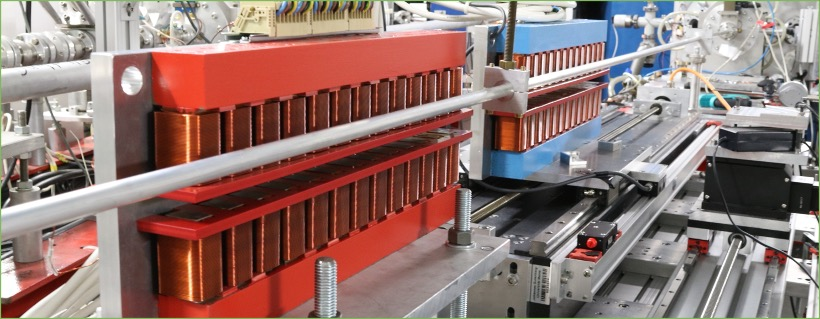
\includegraphics[width=0.8\linewidth]{image/1-1.jpg}\\
  \caption{サンプルの図}
  \label{sample_image}
\end{figure}

\begin{itemize}
  \item a
\end{itemize}
\begin{enumerate}
  \item b
\end{enumerate}

\begin{align}
\frac{1}{2} = \qty(\frac{1}{3}) + \qty{1}\Sigma
\end{align}
\end{document}